% CSE 573 Fall 2026 -- Group 34 -- Project 15 proposal.
% Course format: A4, 1-inch margins, 12pt Times New Roman, single column, PDF.
% Compile: tectonic proposal/proposal.tex
\documentclass[12pt,a4paper]{article}

\usepackage[a4paper,margin=1in]{geometry}
\usepackage{fontspec}
\setmainfont{Times New Roman}
\usepackage{microtype}
\usepackage{booktabs}
\usepackage{array}
\usepackage{tabularx}
\usepackage{needspace}
\usepackage{enumitem}
\usepackage{xcolor}
\usepackage{titlesec}
\usepackage{tikz}
\usetikzlibrary{positioning,arrows.meta,fit,backgrounds}
\usepackage[hidelinks]{hyperref}

\definecolor{accent}{HTML}{1F3A5F}
\definecolor{band}{HTML}{E8EDF3}

\setlist{itemsep=1pt,topsep=2pt,parsep=0pt,leftmargin=*}
\setlength{\parindent}{0pt}
\setlength{\parskip}{3pt}
\renewcommand{\arraystretch}{1.12}

\titleformat{\section}{\normalfont\bfseries\color{accent}}{\thesection.}{0.5em}{}[{\color{accent}\titlerule[0.5pt]}]
\titlespacing*{\section}{0pt}{8pt}{4pt}
\titleformat{\subsection}{\normalfont\bfseries\itshape}{\thesubsection}{0.5em}{}
\titlespacing*{\subsection}{0pt}{4pt}{2pt}
\titleformat{\paragraph}[runin]{\normalfont\bfseries}{}{0pt}{}[.]
\titlespacing*{\paragraph}{0pt}{0pt}{0.5em}

\newcommand{\RQ}[1]{\textbf{RQ#1}}
\newcolumntype{P}[1]{>{\raggedright\arraybackslash}p{#1}}
\newcolumntype{Y}{>{\raggedright\arraybackslash}X}
\newcommand{\hdr}{\rowcolor{band}}
\usepackage{colortbl}

\begin{document}

%------------------------------------------------------------------ title block
\begin{center}
{\bfseries\color{accent} LexGraph: Proof-Carrying Legal Reasoning from Facts\\
to Authorities, Elements and Outcomes}\\[5pt]
Siddharth Axaykumar Mehta \quad\textbullet\quad Om Patel\\[1pt]
CSE 573, Fall 2026 \quad\textbullet\quad Group 34 \quad\textbullet\quad Project 15: Legal AI -- Agentic Law
\end{center}
\vspace{-4pt}\noindent\rule{\textwidth}{0.6pt}

%------------------------------------------------------------------ abstract
\section*{Abstract}
Language models cite cases that do not exist, and outcome predictors can score well simply by reading
the verdict. LexGraph takes only the \emph{facts} of a
dispute, as a lawyer holds them before any judgment exists, and returns (i)~the statutes and precedents
that apply, (ii)~element-level support and refutation, each backed by a verbatim quote, and (iii)~an
outcome estimate with a trace. Every authority and every quotation is checked deterministically against
the corpus before it is shown. We work on all 26,688 Indian Supreme Court judgments (1950--2025),
concentrating on 6,954 land and property disputes. Preliminary held-out results show that facts
alone retrieve precedents at 7.4× a popularity control and statutes at 1.9× the strongest
baseline; that the input construction used by published outcome-prediction work inflates AUROC by
+0.11 to +0.18 through residual disposition language; and that projecting facts onto an authored
element ontology loses outcome signal that a data-induced basis keeps. The remaining work is
gold-standard evaluation, signed-graph authority ranking, graph pattern mining and a verifiable demo.

\textbf{Keywords:} legal AI, proof-carrying reasoning, signed citation graph, ontology-directed
extraction, precedent retrieval, leakage, Indian Supreme Court.

%------------------------------------------------------------------ 1
\section{Problem Definition}
In practice a lawyer holds facts and evidence, never a decided judgment. The task is therefore:

\begin{center}
\fcolorbox{accent}{band}{\parbox{0.94\textwidth}{\centering
\textbf{Given the facts of a land or property dispute:} Step~1, predict the statutes and precedents
that govern it; Step~2, map facts and authorities to the elements of each claim and say which facts
satisfy or defeat which element; Step~3, estimate the outcome, with every output traceable to the record.}}
\end{center}

Following the course description of a proof-carrying system over a signed proof graph, we make two
commitments that separate it from a fluent but unverifiable answer: \textbf{no authority is shown unless it resolves to a real, earlier judgment in the
corpus}, and \textbf{no ``satisfied'' verdict is accepted unless its supporting quote occurs verbatim
in the facts shown}.

\begin{center}
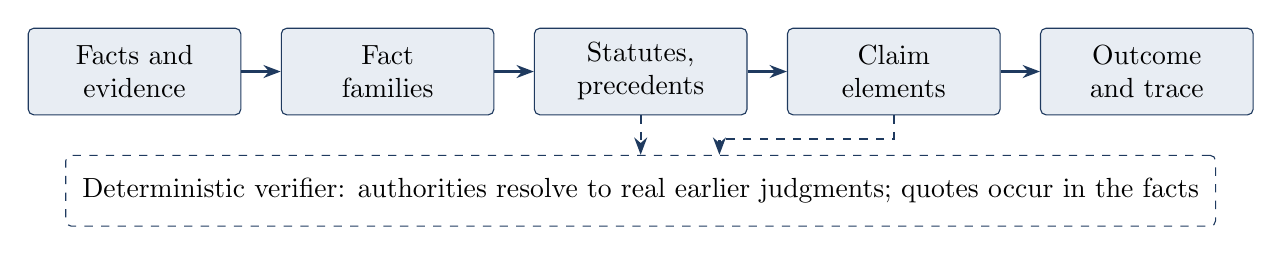
\begin{tikzpicture}[
  node distance=5mm,
  stage/.style={draw=accent,fill=band,rounded corners=2pt,minimum height=11mm,minimum width=27mm,
                align=center,inner sep=2pt},
  arr/.style={-{Stealth[length=2.2mm]},thick,accent}]
  \node[stage] (f) {Facts and\\evidence};
  \node[stage,right=of f] (s2) {Fact\\families};
  \node[stage,right=of s2] (a) {Statutes,\\precedents};
  \node[stage,right=of a] (e) {Claim\\elements};
  \node[stage,right=of e] (o) {Outcome\\and trace};
  \draw[arr] (f)--(s2); \draw[arr] (s2)--(a); \draw[arr] (a)--(e); \draw[arr] (e)--(o);
  \node[draw=accent,dashed,rounded corners=2pt,minimum height=9mm,align=center,
        below=5mm of a,inner xsep=6pt]
        (v) {Deterministic verifier: authorities resolve to real earlier judgments; quotes occur in the facts};
  \draw[arr,dashed] (a.south)--(v.north -| a);
  \draw[arr,dashed] (e.south)--++(0,-3mm) -| ([xshift=10mm]v.north);
\end{tikzpicture}
\end{center}

We pursue four research questions.
\begin{enumerate}[label=\RQ{\arabic*}.,leftmargin=2.6em]
\item How much of the apparent predictability of court outcomes comes from the facts, from the court's
reasoning, and from disposition language that survives masking?
\item Do facts alone retrieve the right statutes and precedents better than controls that exploit
citation skew or copy text?
\item Does ontology-directed symbolic structure (claims, elements) preserve outcome signal compared with
a data-induced representation, and can it still serve as a checkable explanation layer?
\item Can a signed citation graph tell whether a retrieved authority is still good law?
\end{enumerate}
We do not claim a deployable outcome predictor.

%------------------------------------------------------------------ 2
\section{Data Sets}
\begin{tabularx}{\textwidth}{@{}P{3.1cm}Y@{}}
\toprule
\hdr \textbf{Resource} & \textbf{Description} \\
\midrule
Legal AI Dataset (provided) &
26,688 Supreme Court of India judgment PDFs, 1950--2025 (6.8~GB, held locally), with Indian Kanoon
citation metadata and a spreadsheet identifying 6,954 land and property disputes: the working corpus,
100\% joined to PDFs, median 5,302 words. Only about 32.5\% of listed ``precedents'' are genuine case
citations, and only 25.6\% of 46,904 case-citation edges point inside the corpus, so recall is always
reported against \emph{reachable} authorities with the raw figure beside it. \\
\addlinespace
Derived resources &
Win/lose labels (two independent labellers on the land subset; 14,168 usable rules-based labels
corpus-wide); 96,623 verbatim-grounded facts; a registry of 42 Acts (58,295 statute citations, 61.4\%
resolved); two splits that group related judgments and forbid time travel, \emph{forum\_heldout} (test
n=902) and \emph{temporal\_2004\_2013} (test n=768); a signed citation graph of 8,467 edges, 62.6\%
carrying a sign (built earlier, to be restored in WP2). \\
\addlinespace
Ontology and gold set &
Provided Land and Property Dispute ontology (15 claims, 66 elements, 6 defence families, 4 remedy tiers); 150 gold cases and 214 element judgements to be annotated in this project. ILDC \cite{ildc} is an optional external check only, as its release is gated. \\
\bottomrule
\end{tabularx}

%------------------------------------------------------------------ 3
\section{State-of-the-Art Methods and Algorithms}
\paragraph{Outcome prediction} Aletras et al.~\cite{aletras} predicted decisions from text with linear models;
Chalkidis et al.~\cite{chalkidis19} and LEGAL-BERT~\cite{legalbert} moved to neural encoders. For India, ILDC~\cite{ildc} introduced court judgment prediction and explanation, with the
best reported accuracy near 78\% on the final 512 tokens. Nigam and Deroy~\cite{nigam} ran facts-only
on ILDC and found it worse. Watson et al.~\cite{watson} show that a model trained on the 4\% of
features flagged as leakage in UK tribunal claims performs strongly, which general shortcut-learning
results~\cite{geirhos} predict.
\paragraph{Ontology and extraction} Sadowski and Chudziak~\cite{sadowski} measure semantic loss when
legal text is ontologised, but do not compare induced and authored vocabularies, the control we run.
\paragraph{Retrieval and graphs} BM25~\cite{bm25}, dense embeddings (Qwen3-Embedding~\cite{qwen3})
and reciprocal rank fusion~\cite{rrf} are the standard retrieval stack; HITS~\cite{hits} and signed
variants rank authorities from citation structure; gSpan~\cite{gspan} mines frequent subgraphs. None of the work above verifies every cited
authority against real citation data or ranks authorities by signed citation polarity.

%------------------------------------------------------------------ 4
\needspace{6\baselineskip}
\section{Research Plan}
\subsection{Groundwork complete (feasibility evidence)}
The pipeline is built and measured on held-out data (48 tests pass); every figure is read from a stored result file.

\begin{tabularx}{\textwidth}{@{}P{3.6cm}Y Y@{}}
\toprule
\hdr \textbf{Stage} & \textbf{Result (held-out)} & \textbf{Control} \\
\midrule
Precedents from facts & Recall@10 0.238 (BM25 + dense, RRF) & Popularity 0.032 (7.4×) \\
Statutes from facts & Micro-F1 0.173 on provisions not named in the text & Claim-family prior 0.093 (1.9×); copy control 0.000 \\
Fact families (soft) & AUROC 0.633 from 345 dimensions & 0.629 from 47,354 text features \\
Element layer & 0.62\% fabricated quotes; 96.9\% test--retest agreement; AUROC 0.521 & Fails acceptance vs soft facts (−0.11, CI excludes 0) \\
Leakage (RQ1) & Final-512 input +0.176 AUROC over facts; boundary near 128 words & Volume-matched windows; all 8 decades \\
Trace faithfulness & Cited facts move the prediction 3.1× as much as random facts & Random and inverse-ranked deletion \\
\bottomrule
\end{tabularx}

\subsection{Classical and modern methods, scored identically}
\begin{tabularx}{\textwidth}{@{}P{2.1cm}Y Y@{}}
\toprule
\hdr \textbf{Task} & \textbf{Classical / baseline} & \textbf{Modern} \\
\midrule
Outcome & Per-decade majority; TF-IDF + logistic regression; gradient boosting on six feature groups & Zero-shot, few-shot and chain-of-thought LLMs (llama4-scout-17b, qwen3-235b) \\
Retrieval & BM25; frequent-itemset and atom-overlap baselines & Dense Qwen3-Embedding-8B; RRF fusion \\
Extraction & Regular-expression citation and statute rules & Ontology-directed LLM grounding with quote verification \\
Graph & In-degree, HITS; flat itemsets (498 mined, none significant after Benjamini--Hochberg) & Signed anco-HITS-style ranking; gSpan over fact--element--claim graphs \\
\bottomrule
\end{tabularx}

\subsection{Remaining work packages}
\begin{description}[leftmargin=0pt,labelindent=0pt,style=unboxed,itemsep=2pt]
\item[WP1 Gold evaluation.] Annotate the 150 cases and 214 element judgements, with both members
annotating 30 shared cases. This gives the first extraction precision, recall and F1, and tests whether
element verdicts are \emph{correct}, not merely well-formed.
\item[WP2 Signed authority ranking.] Restore the signed graph, rank retrieved precedents by
proof-support and edge polarity, and test whether it flags overruled or distinguished authorities
better than in-degree. Only 174 of 8,467 edges are negative, so we expect a modest effect and will say so.
\item[WP3 Claim-family patterns.] Cluster facts per claim family; mine graph patterns with gSpan.
\item[WP4 Proof graph and verifier.] Connect facts, elements, authorities and outcome into one graph with
support, refutation and decisive-fact edges, and certify or refuse each authority and quote.
\item[WP5 Demo.] A web dashboard where a user pastes facts and sees certified authorities, element
verdicts with quotes, and the trace.
\end{description}

%------------------------------------------------------------------ 5
\section{Evaluation Plan}
Each stage is scored on its own task, win/lose last, and every number needs a control: popularity
(precedents), copy-from-text (statutes), per-decade majority (outcomes), volume-matched windows (leakage).

\begin{tabularx}{\textwidth}{@{}P{3.1cm}Y@{}}
\toprule
\hdr \textbf{Aspect} & \textbf{Protocol} \\
\midrule
Splits & \emph{forum\_heldout} and \emph{temporal\_2004\_2013}; every result file records its split hash. \\
Outcome & Accuracy, macro-F1, AUROC and calibration (ECE) with paired-bootstrap 95\% confidence intervals; McNemar tests for paired classifiers. \\
Retrieval & Recall@\emph{k}, MRR and nDCG@10 against reachable authorities, with a check that each result pre-dates the query. \\
Extraction, elements & Per-class precision and recall against gold, Cohen's κ between the two annotators, and the 3.1\% self-disagreement of repeated model runs as the floor. \\
Verification & Share of displayed authorities that resolve to a corpus judgment; share of quotes refused by the quote gate. \\
\bottomrule
\end{tabularx}

\paragraph{Targets} Recall@10 ≥ 0.20; quote fabrication ≤ 1\%; inter-annotator κ ≥ 0.6; and a
reported confidence interval for signed ranking against in-degree, whichever way it falls.
\paragraph{Risks} Outcome AUROC may stay near chance (every confidence interval spans about 0.11), the vocabulary is
20.3\% out-of-vocabulary against a 5\% freeze threshold, and certification proves provenance, not
relevance, so the demo reports both.

%------------------------------------------------------------------ 6
\needspace{5\baselineskip}
\section{Project Timeline}
\begin{tabularx}{\textwidth}{@{}P{3.2cm}Y@{}}
\toprule
\hdr \textbf{Dates (2026)} & \textbf{Task and deliverable} \\
\midrule
Oct 7--21 & Proposal; freeze splits; WP1 gold annotation, extraction P/R/F1, κ \\
Oct 14--28 & WP2 signed graph restored; ranking vs in-degree and HITS \\
Oct 21--Nov 11 & Element correctness against gold; WP3 gSpan patterns per claim family \\
Oct 28--Nov 18 & Class presentation in assigned slot (slides ready by Oct 26) \\
Nov 4--20 & WP4 proof graph, verifier and trace integration \\
Nov 9--22 & WP5 dashboard; end-to-end test on 10 unseen post-2000 cases \\
Nov 23--Dec 2 & Group demo; code and data freeze \\
Dec 2--9 & Final report (15--20 pages) with supplemental code and data, due Dec 9 \\
\bottomrule
\end{tabularx}

%------------------------------------------------------------------ 7
\section{Division of Work}
\begin{tabularx}{\textwidth}{@{}P{4.6cm}Y@{}}
\toprule
\hdr \textbf{Member} & \textbf{Responsibility} \\
\midrule
Siddharth Axaykumar Mehta & Pipeline, retrieval, signed graph (WP2), proof graph and verifier (WP4), outcome models and statistics \\
Om Patel & Gold annotation and element correctness (WP1), patterns (WP3), dashboard (WP5), presentation \\
Both & Half the gold set each (30 cases shared); weekly meeting; contribution log in the repository; final report \\
\bottomrule
\end{tabularx}

%------------------------------------------------------------------ references
\begin{thebibliography}{99}
\setlength{\itemsep}{0pt}\setlength{\parsep}{0pt}\setlength{\parskip}{0pt}
\bibitem{aletras} N. Aletras et al. Predicting judicial decisions of the ECtHR. \emph{PeerJ CS}, 2016.
\bibitem{chalkidis19} I. Chalkidis, I. Androutsopoulos, N. Aletras. Neural legal judgment prediction in English. \emph{ACL}, 2019.
\bibitem{legalbert} I. Chalkidis et al. LEGAL-BERT: the muppets straight out of law school. \emph{Findings of EMNLP}, 2020.
\bibitem{ildc} V. Malik et al. ILDC for CJPE: Indian legal documents corpus for court judgment prediction and explanation. \emph{ACL-IJCNLP}, 2021.
\bibitem{nigam} S. K. Nigam, A. Deroy. Fact-based court judgment prediction. arXiv:2311.13350, 2023.
\bibitem{watson} J. Watson et al. Shortcut learning in legal judgment prediction: empirical evidence from the UK Employment Tribunal. arXiv:2607.04261, 2026.
\bibitem{geirhos} R. Geirhos et al. Shortcut learning in deep neural networks. \emph{Nat. Mach. Intell.}, 2020.
\bibitem{sadowski} A. Sadowski, J. A. Chudziak. On measuring semantic preservation in legal ontology learning. arXiv:2608.12326, 2026.
\bibitem{bm25} S. Robertson, H. Zaragoza. The probabilistic relevance framework: BM25 and beyond. \emph{Found. Trends IR}, 2009.
\bibitem{qwen3} Y. Zhang et al. Qwen3 Embedding: advancing text embedding and reranking through foundation models. arXiv:2506.05176, 2025.
\bibitem{rrf} G. Cormack, C. Clarke, S. Buettcher. Reciprocal rank fusion outperforms Condorcet and individual rank learning methods. \emph{SIGIR}, 2009.
\bibitem{hits} J. Kleinberg. Authoritative sources in a hyperlinked environment. \emph{JACM}, 1999.
\bibitem{gspan} X. Yan, J. Han. gSpan: graph-based substructure pattern mining. \emph{ICDM}, 2002.
\end{thebibliography}

\end{document}
